\documentclass[twoside]{book}

% Packages required by doxygen
\usepackage{fixltx2e}
\usepackage{calc}
\usepackage{doxygen}
\usepackage{graphicx}
\usepackage[utf8]{inputenc}
\usepackage{makeidx}
\usepackage{multicol}
\usepackage{multirow}
\PassOptionsToPackage{warn}{textcomp}
\usepackage{textcomp}
\usepackage[nointegrals]{wasysym}
\usepackage[table]{xcolor}

% Font selection
\usepackage[T1]{fontenc}
\usepackage{mathptmx}
\usepackage[scaled=.90]{helvet}
\usepackage{courier}
\usepackage{amssymb}
\usepackage{sectsty}
\renewcommand{\familydefault}{\sfdefault}
\allsectionsfont{%
  \fontseries{bc}\selectfont%
  \color{darkgray}%
}
\renewcommand{\DoxyLabelFont}{%
  \fontseries{bc}\selectfont%
  \color{darkgray}%
}
\newcommand{\+}{\discretionary{\mbox{\scriptsize$\hookleftarrow$}}{}{}}

% Page & text layout
\usepackage{geometry}
\geometry{%
  a4paper,%
  top=2.5cm,%
  bottom=2.5cm,%
  left=2.5cm,%
  right=2.5cm%
}
\tolerance=750
\hfuzz=15pt
\hbadness=750
\setlength{\emergencystretch}{15pt}
\setlength{\parindent}{0cm}
\setlength{\parskip}{0.2cm}
\makeatletter
\renewcommand{\paragraph}{%
  \@startsection{paragraph}{4}{0ex}{-1.0ex}{1.0ex}{%
    \normalfont\normalsize\bfseries\SS@parafont%
  }%
}
\renewcommand{\subparagraph}{%
  \@startsection{subparagraph}{5}{0ex}{-1.0ex}{1.0ex}{%
    \normalfont\normalsize\bfseries\SS@subparafont%
  }%
}
\makeatother

% Headers & footers
\usepackage{fancyhdr}
\pagestyle{fancyplain}
\fancyhead[LE]{\fancyplain{}{\bfseries\thepage}}
\fancyhead[CE]{\fancyplain{}{}}
\fancyhead[RE]{\fancyplain{}{\bfseries\leftmark}}
\fancyhead[LO]{\fancyplain{}{\bfseries\rightmark}}
\fancyhead[CO]{\fancyplain{}{}}
\fancyhead[RO]{\fancyplain{}{\bfseries\thepage}}
\fancyfoot[LE]{\fancyplain{}{}}
\fancyfoot[CE]{\fancyplain{}{}}
\fancyfoot[RE]{\fancyplain{}{\bfseries\scriptsize Generated on Thu Jun 2 2016 15\+:31\+:29 for L\+K\+M hd44780 lcd by Doxygen }}
\fancyfoot[LO]{\fancyplain{}{\bfseries\scriptsize Generated on Thu Jun 2 2016 15\+:31\+:29 for L\+K\+M hd44780 lcd by Doxygen }}
\fancyfoot[CO]{\fancyplain{}{}}
\fancyfoot[RO]{\fancyplain{}{}}
\renewcommand{\footrulewidth}{0.4pt}
\renewcommand{\chaptermark}[1]{%
  \markboth{#1}{}%
}
\renewcommand{\sectionmark}[1]{%
  \markright{\thesection\ #1}%
}

% Indices & bibliography
\usepackage{natbib}
\usepackage[titles]{tocloft}
\setcounter{tocdepth}{3}
\setcounter{secnumdepth}{5}
\makeindex

% Hyperlinks (required, but should be loaded last)
\usepackage{ifpdf}
\ifpdf
  \usepackage[pdftex,pagebackref=true]{hyperref}
\else
  \usepackage[ps2pdf,pagebackref=true]{hyperref}
\fi
\hypersetup{%
  colorlinks=true,%
  linkcolor=blue,%
  citecolor=blue,%
  unicode%
}

% Custom commands
\newcommand{\clearemptydoublepage}{%
  \newpage{\pagestyle{empty}\cleardoublepage}%
}


%===== C O N T E N T S =====

\begin{document}

% Titlepage & ToC
\hypersetup{pageanchor=false,
             bookmarks=true,
             bookmarksnumbered=true,
             pdfencoding=unicode
            }
\pagenumbering{roman}
\begin{titlepage}
\vspace*{7cm}
\begin{center}%
{\Large L\+K\+M hd44780 lcd \\[1ex]\large 0.\+1 }\\
\vspace*{1cm}
{\large Generated by Doxygen 1.8.8}\\
\vspace*{0.5cm}
{\small Thu Jun 2 2016 15:31:29}\\
\end{center}
\end{titlepage}
\clearemptydoublepage
\tableofcontents
\clearemptydoublepage
\pagenumbering{arabic}
\hypersetup{pageanchor=true}

%--- Begin generated contents ---
\chapter{lcd-\/kernel-\/driver}
\label{md__home_pi_SysProg_lcd-driver_README}
\hypertarget{md__home_pi_SysProg_lcd-driver_README}{}
lcd kernel driver for 16x2 H\+D44780

helpful link to compile a kernel module\+: \href{https://github.com/diederikdehaas/cknow.org/blob/master/rpi/compile-kernel-module-on-raspberrypi.md}{\tt https\+://github.\+com/diederikdehaas/cknow.\+org/blob/master/rpi/compile-\/kernel-\/module-\/on-\/raspberrypi.\+md} 
\chapter{File Index}
\section{File List}
Here is a list of all files with brief descriptions\+:\begin{DoxyCompactList}
\item\contentsline{section}{/home/pi/\+Sys\+Prog/lcd-\/driver/\hyperlink{hd44780_8c}{hd44780.\+c} \\*Loadable kernel module character device driver for support a simple 2x16 lcd display. within the lcd display is a commonly used H\+D44780 controller implemented }{\pageref{hd44780_8c}}{}
\item\contentsline{section}{/home/pi/\+Sys\+Prog/lcd-\/driver/\hyperlink{hd44780_8mod_8c}{hd44780.\+mod.\+c} }{\pageref{hd44780_8mod_8c}}{}
\item\contentsline{section}{/home/pi/\+Sys\+Prog/lcd-\/driver/\hyperlink{ioctl__header_8h}{ioctl\+\_\+header.\+h} }{\pageref{ioctl__header_8h}}{}
\item\contentsline{section}{/home/pi/\+Sys\+Prog/lcd-\/driver/\hyperlink{usr-lcd-control_8c}{usr-\/lcd-\/control.\+c} \\*Linux user space program that communicates with the hd44780 linux kernel module (L\+K\+M). to work with the device the /dev/hd44780 must be called }{\pageref{usr-lcd-control_8c}}{}
\item\contentsline{section}{/home/pi/\+Sys\+Prog/lcd-\/driver/\hyperlink{usr-print-ip_8c}{usr-\/print-\/ip.\+c} }{\pageref{usr-print-ip_8c}}{}
\end{DoxyCompactList}

\chapter{File Documentation}
\hypertarget{hd44780_8c}{\section{/home/pi/\+Sys\+Prog/lcd-\/driver/hd44780.c File Reference}
\label{hd44780_8c}\index{/home/pi/\+Sys\+Prog/lcd-\/driver/hd44780.\+c@{/home/pi/\+Sys\+Prog/lcd-\/driver/hd44780.\+c}}
}


loadable kernel module character device driver for support a simple 2x16 lcd display. within the lcd display is a commonly used H\+D44780 controller implemented.  


{\ttfamily \#include $<$linux/module.\+h$>$}\\*
{\ttfamily \#include $<$linux/moduleparam.\+h$>$}\\*
{\ttfamily \#include $<$linux/kernel.\+h$>$}\\*
{\ttfamily \#include $<$linux/init.\+h$>$}\\*
{\ttfamily \#include $<$linux/fs.\+h$>$}\\*
{\ttfamily \#include $<$linux/cdev.\+h$>$}\\*
{\ttfamily \#include $<$linux/types.\+h$>$}\\*
{\ttfamily \#include $<$linux/device.\+h$>$}\\*
{\ttfamily \#include $<$linux/gpio.\+h$>$}\\*
{\ttfamily \#include $<$linux/delay.\+h$>$}\\*
{\ttfamily \#include $<$linux/ctype.\+h$>$}\\*
{\ttfamily \#include $<$asm/uaccess.\+h$>$}\\*
{\ttfamily \#include $<$asm/errno.\+h$>$}\\*
{\ttfamily \#include $<$linux/wait.\+h$>$}\\*
{\ttfamily \#include $<$linux/hrtimer.\+h$>$}\\*
{\ttfamily \#include $<$linux/ktime.\+h$>$}\\*
{\ttfamily \#include $<$linux/interrupt.\+h$>$}\\*
{\ttfamily \#include \char`\"{}ioctl\+\_\+header.\+h\char`\"{}}\\*
Include dependency graph for hd44780.\+c\+:\nopagebreak
\begin{figure}[H]
\begin{center}
\leavevmode
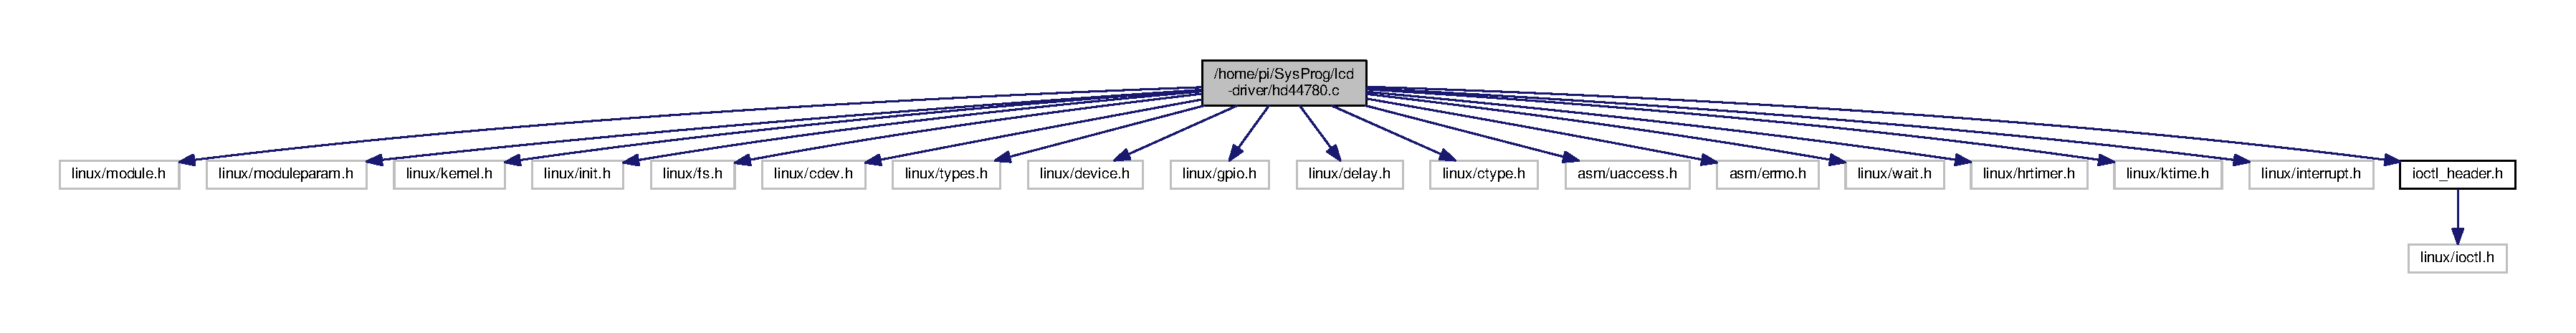
\includegraphics[width=350pt]{hd44780_8c__incl}
\end{center}
\end{figure}
\subsection*{Functions}
\begin{DoxyCompactItemize}
\item 
\hyperlink{hd44780_8c_a96387bbd4c7b27256a28863012f6c485}{M\+O\+D\+U\+L\+E\+\_\+\+A\+U\+T\+H\+O\+R} (\char`\"{}Daniel Obermaier $<$mailto\+:dan.\+obermaier@gmail.\+com$>$, Victor Nagy $<$mailto\+:victor.\+nagy@hotmail.\+de$>$\char`\"{})
\begin{DoxyCompactList}\small\item\em $<$ core header for loading L\+K\+Ms into the kernel \end{DoxyCompactList}\item 
\hyperlink{hd44780_8c_a3b308580fb76459a08a77c2394250426}{M\+O\+D\+U\+L\+E\+\_\+\+D\+E\+S\+C\+R\+I\+P\+T\+I\+O\+N} (\char`\"{}driver for L\+C\+D Display with H\+D44780 controller\char`\"{})
\item 
\hyperlink{hd44780_8c_ad94b36675e7eb067ea3ce6ff9e244a44}{M\+O\+D\+U\+L\+E\+\_\+\+L\+I\+C\+E\+N\+S\+E} (\char`\"{}G\+P\+L\char`\"{})
\item 
\hyperlink{hd44780_8c_a4b75c2cb371865e62f06fc635df9401e}{M\+O\+D\+U\+L\+E\+\_\+\+V\+E\+R\+S\+I\+O\+N} (\char`\"{}0.\+1\char`\"{})
\item 
static void \hyperlink{hd44780_8c_a0eab6f129d21added23841a39571dea3}{write\+\_\+nibble} (int regist, int value)
\begin{DoxyCompactList}\small\item\em writes 4-\/bit values to gpio \end{DoxyCompactList}\item 
static void \hyperlink{hd44780_8c_ae0b6133b70bc190065133c49eb16f55f}{write\+\_\+lcd} (int regist, int value)
\begin{DoxyCompactList}\small\item\em uses write\+\_\+nibble to shift and reverse logic values \end{DoxyCompactList}\item 
static int \hyperlink{hd44780_8c_abedd5fbc5004aefc727091a522a79391}{gpio\+\_\+request\+\_\+output} (int nr)
\begin{DoxyCompactList}\small\item\em checks if gpio can be written successfully \end{DoxyCompactList}\item 
static int \hyperlink{hd44780_8c_aaeb9d01b89561b7086b450105ecd32fe}{exit\+\_\+display} (void)
\begin{DoxyCompactList}\small\item\em frees memory on every initialized gpio pin if module gets unloaded from kernel \end{DoxyCompactList}\item 
static void \+\_\+\+\_\+exit \hyperlink{hd44780_8c_a39f7f81eb9dcc1767834f259f32979ba}{mod\+\_\+exit} (void)
\begin{DoxyCompactList}\small\item\em lkm exit function \end{DoxyCompactList}\item 
static int \+\_\+\+\_\+init \hyperlink{hd44780_8c_a56a4067c846fe4fc7959a60d87b8b0f1}{init\+\_\+display} (void)
\begin{DoxyCompactList}\small\item\em initializes display as soon as the module is loaded into the kernel \end{DoxyCompactList}\item 
static int \hyperlink{hd44780_8c_aa1ec1faa20fcdd72008800756f5f5134}{dev\+\_\+open} (struct inode $\ast$inode, struct file $\ast$fp)
\begin{DoxyCompactList}\small\item\em executed from user via userspace interface program and increment device counter \end{DoxyCompactList}\item 
static int \hyperlink{hd44780_8c_a6b207bce4fc5e05120e630d1c4bb6377}{dev\+\_\+release} (struct inode $\ast$inode, struct file $\ast$fp)
\begin{DoxyCompactList}\small\item\em executed from user via userspace interface program and decrement device counter \end{DoxyCompactList}\item 
static ssize\+\_\+t \hyperlink{hd44780_8c_a23ebf6135f28b8d3c3e693971b9e2333}{dev\+\_\+write} (struct file $\ast$instance, const char \+\_\+\+\_\+user $\ast$user, size\+\_\+t cnt, loff\+\_\+t $\ast$offset)
\begin{DoxyCompactList}\small\item\em function is called when device is being written from user space \end{DoxyCompactList}\item 
\hyperlink{hd44780_8c_a1dc5174a07767c41761c513b9ba16422}{module\+\_\+param} (\hyperlink{hd44780_8c_ac8947941479c38403a09c14a60b03f01}{major}, int, S\+\_\+\+I\+R\+U\+G\+O$\vert$S\+\_\+\+I\+W\+U\+S\+R)
\item 
\hyperlink{hd44780_8c_aa3d8ce5316766e98caada6c877ded662}{module\+\_\+param} (\hyperlink{hd44780_8c_ad43c3812e6d13e0518d9f8b8f463ffcf}{count}, int, S\+\_\+\+I\+R\+U\+G\+O$\vert$S\+\_\+\+I\+W\+U\+S\+R)
\item 
static int \+\_\+\+\_\+init \hyperlink{hd44780_8c_a2b796de854877d3b6e8e9c73a8c60c00}{mod\+\_\+init} (void)
\begin{DoxyCompactList}\small\item\em kernel module initialization function \end{DoxyCompactList}\item 
\hyperlink{hd44780_8c_a63936a07c493d98700dad3cf37aa30de}{module\+\_\+init} (\hyperlink{hd44780_8c_a2b796de854877d3b6e8e9c73a8c60c00}{mod\+\_\+init})
\begin{DoxyCompactList}\small\item\em a module must use the \hyperlink{hd44780_8c_a63936a07c493d98700dad3cf37aa30de}{module\+\_\+init()} and \hyperlink{hd44780_8c_a92f7251a3e21772c1063cb378ab99b3d}{module\+\_\+exit()} macros from linux/init.\+h \end{DoxyCompactList}\item 
\hyperlink{hd44780_8c_a92f7251a3e21772c1063cb378ab99b3d}{module\+\_\+exit} (\hyperlink{hd44780_8c_a39f7f81eb9dcc1767834f259f32979ba}{mod\+\_\+exit})
\end{DoxyCompactItemize}
\subsection*{Variables}
\begin{DoxyCompactItemize}
\item 
static int \hyperlink{hd44780_8c_ac8947941479c38403a09c14a60b03f01}{major} = 0
\begin{DoxyCompactList}\small\item\em major number as an lkm identifier \end{DoxyCompactList}\item 
static int \hyperlink{hd44780_8c_aec7b96885baf2e6f10efbdef9d935a0b}{minor} = 0
\item 
static int \hyperlink{hd44780_8c_ad43c3812e6d13e0518d9f8b8f463ffcf}{count} = 1
\item 
dev\+\_\+t \hyperlink{hd44780_8c_a8910285a0352a5c710e65ec9ecbe32a1}{dev} = 0
\begin{DoxyCompactList}\small\item\em variable for lcd device \end{DoxyCompactList}\item 
static int \hyperlink{hd44780_8c_afd20d9c5f02b616c3c3cb41892e3f5d3}{dev\+\_\+cnt} = 0
\begin{DoxyCompactList}\small\item\em used to prevent multiple access \end{DoxyCompactList}\item 
static struct cdev $\ast$ \hyperlink{hd44780_8c_a628c122c638ae60b0c6d8a30c4e55b46}{driver\+\_\+object}
\item 
static struct class $\ast$ \hyperlink{hd44780_8c_a2924ecef65e0b40dc3dfab97f5a18b2f}{hd44780\+\_\+class}
\item 
static struct device $\ast$ \hyperlink{hd44780_8c_a7f39d148808b935cc26697ba64f38127}{hd44780\+\_\+dev}
\item 
static char \hyperlink{hd44780_8c_a21566485093f5feef65ee0fc7a32a91e}{textbuffer} \mbox{[}1024\mbox{]}
\item 
static struct file\+\_\+operations \hyperlink{hd44780_8c_a28ee7ed9613033920e733c9da671f79c}{fops}
\begin{DoxyCompactList}\small\item\em Devices are represented as file structures in the kernel. \end{DoxyCompactList}\end{DoxyCompactItemize}


\subsection{Detailed Description}
loadable kernel module character device driver for support a simple 2x16 lcd display. within the lcd display is a commonly used H\+D44780 controller implemented. 

\begin{DoxyAuthor}{Author}
Daniel Obermaier Victor Nagy Markus Fischer 
\end{DoxyAuthor}
\begin{DoxyDate}{Date}
01. June 2016 
\end{DoxyDate}
\begin{DoxyVersion}{Version}
0.\+1 
\end{DoxyVersion}
\begin{DoxySeeAlso}{See also}
\href{https://www.sparkfun.com/datasheets/LCD/HD44780.pdf}{\tt https\+://www.\+sparkfun.\+com/datasheets/\+L\+C\+D/\+H\+D44780.\+pdf} datasheet for this hd44780 controller 
\end{DoxySeeAlso}


\subsection{Function Documentation}
\hypertarget{hd44780_8c_aa1ec1faa20fcdd72008800756f5f5134}{\index{hd44780.\+c@{hd44780.\+c}!dev\+\_\+open@{dev\+\_\+open}}
\index{dev\+\_\+open@{dev\+\_\+open}!hd44780.\+c@{hd44780.\+c}}
\subsubsection[{dev\+\_\+open}]{\setlength{\rightskip}{0pt plus 5cm}static int dev\+\_\+open (
\begin{DoxyParamCaption}
\item[{struct inode $\ast$}]{inode, }
\item[{struct file $\ast$}]{fp}
\end{DoxyParamCaption}
)\hspace{0.3cm}{\ttfamily [static]}}}\label{hd44780_8c_aa1ec1faa20fcdd72008800756f5f5134}


executed from user via userspace interface program and increment device counter 

will be called if device will be opened 
\begin{DoxyParams}{Parameters}
{\em inode} & to device file \\
\hline
{\em pointer} & to device file \\
\hline
\end{DoxyParams}

\begin{DoxyCode}
297                                                          \{
298     printk(KERN\_INFO \textcolor{stringliteral}{"hd44780: device opened from user\(\backslash\)n"});
299 
300     \hyperlink{hd44780_8c_afd20d9c5f02b616c3c3cb41892e3f5d3}{dev\_cnt}++;   \textcolor{comment}{//increment counter }
301 
302     \textcolor{keywordflow}{return} 0;   
303 \}
\end{DoxyCode}
\hypertarget{hd44780_8c_a6b207bce4fc5e05120e630d1c4bb6377}{\index{hd44780.\+c@{hd44780.\+c}!dev\+\_\+release@{dev\+\_\+release}}
\index{dev\+\_\+release@{dev\+\_\+release}!hd44780.\+c@{hd44780.\+c}}
\subsubsection[{dev\+\_\+release}]{\setlength{\rightskip}{0pt plus 5cm}static int dev\+\_\+release (
\begin{DoxyParamCaption}
\item[{struct inode $\ast$}]{inode, }
\item[{struct file $\ast$}]{fp}
\end{DoxyParamCaption}
)\hspace{0.3cm}{\ttfamily [static]}}}\label{hd44780_8c_a6b207bce4fc5e05120e630d1c4bb6377}


executed from user via userspace interface program and decrement device counter 

will be called on closing the device 
\begin{DoxyParams}{Parameters}
{\em inode} & to device file \\
\hline
{\em pointer} & to device file \\
\hline
\end{DoxyParams}

\begin{DoxyCode}
312                                                             \{
313     printk(KERN\_INFO \textcolor{stringliteral}{"hd44780: device closed from user\(\backslash\)n"});
314 
315     \hyperlink{hd44780_8c_afd20d9c5f02b616c3c3cb41892e3f5d3}{dev\_cnt}--;   \textcolor{comment}{//decrement counter}
316 
317     \textcolor{keywordflow}{return} 0;
318 \}
\end{DoxyCode}
\hypertarget{hd44780_8c_a23ebf6135f28b8d3c3e693971b9e2333}{\index{hd44780.\+c@{hd44780.\+c}!dev\+\_\+write@{dev\+\_\+write}}
\index{dev\+\_\+write@{dev\+\_\+write}!hd44780.\+c@{hd44780.\+c}}
\subsubsection[{dev\+\_\+write}]{\setlength{\rightskip}{0pt plus 5cm}static ssize\+\_\+t dev\+\_\+write (
\begin{DoxyParamCaption}
\item[{struct file $\ast$}]{instance, }
\item[{const char \+\_\+\+\_\+user $\ast$}]{user, }
\item[{size\+\_\+t}]{cnt, }
\item[{loff\+\_\+t $\ast$}]{offset}
\end{DoxyParamCaption}
)\hspace{0.3cm}{\ttfamily [static]}}}\label{hd44780_8c_a23ebf6135f28b8d3c3e693971b9e2333}


function is called when device is being written from user space 


\begin{DoxyParams}{Parameters}
{\em pointer} & to a file instance \\
\hline
{\em buffer} & contains the string to write onto the device \\
\hline
{\em size} & of array that is being passed in the const char buffer \\
\hline
{\em offset} & if required \\
\hline
\end{DoxyParams}
\begin{DoxyReturn}{Returns}
number of characters left 
\end{DoxyReturn}

\begin{DoxyCode}
330                                                                                                     \{
331 
332     \textcolor{keywordtype}{unsigned} \textcolor{keywordtype}{long} not\_copied; 
333     \textcolor{keywordtype}{unsigned} \textcolor{keywordtype}{long} to\_copy;
334     \textcolor{keywordtype}{int} i;
335 
336     \textcolor{keywordtype}{char} msg\_from\_user[128] = \{ 0 \};
337 
338     to\_copy = min(cnt, \textcolor{keyword}{sizeof}(\hyperlink{hd44780_8c_a21566485093f5feef65ee0fc7a32a91e}{textbuffer}));
339     not\_copied = copy\_from\_user(\hyperlink{hd44780_8c_a21566485093f5feef65ee0fc7a32a91e}{textbuffer}, user, to\_copy);
340 
341     \hyperlink{hd44780_8c_ae0b6133b70bc190065133c49eb16f55f}{write\_lcd}(0, 0x80);        \textcolor{comment}{//set cursor to begin}
342 
343     \textcolor{keywordflow}{for}(i = 0; i < to\_copy && \hyperlink{hd44780_8c_a21566485093f5feef65ee0fc7a32a91e}{textbuffer}[i]; i++)\{
344         \textcolor{keywordflow}{if}(isprint(textbuffer[i]))\{         \textcolor{comment}{//checks, whether the passed character is printable }
345             \hyperlink{hd44780_8c_ae0b6133b70bc190065133c49eb16f55f}{write\_lcd}(1, textbuffer[i]);
346         \}
347         \textcolor{keywordflow}{if}( i == 15)\{
348             \hyperlink{hd44780_8c_ae0b6133b70bc190065133c49eb16f55f}{write\_lcd}(0, 0xc0);            \textcolor{comment}{//jump to second row of display}
349         \}
350     \}
351 
352     \textcolor{keywordflow}{if}(copy\_from\_user(msg\_from\_user, user, cnt)) \{
353         printk(\textcolor{stringliteral}{"failed copy from user"});
354     \}
355 \textcolor{keywordflow}{return} to\_copy-not\_copied;              \textcolor{comment}{//returns how many characters are left -> returns 0 if everything
       is copied properly }
356 \}
\end{DoxyCode}
\hypertarget{hd44780_8c_aaeb9d01b89561b7086b450105ecd32fe}{\index{hd44780.\+c@{hd44780.\+c}!exit\+\_\+display@{exit\+\_\+display}}
\index{exit\+\_\+display@{exit\+\_\+display}!hd44780.\+c@{hd44780.\+c}}
\subsubsection[{exit\+\_\+display}]{\setlength{\rightskip}{0pt plus 5cm}static int exit\+\_\+display (
\begin{DoxyParamCaption}
\item[{void}]{}
\end{DoxyParamCaption}
)\hspace{0.3cm}{\ttfamily [static]}}}\label{hd44780_8c_aaeb9d01b89561b7086b450105ecd32fe}


frees memory on every initialized gpio pin if module gets unloaded from kernel 

called from kernel callbacks 
\begin{DoxyCode}
279                              \{
280     printk(\textcolor{stringliteral}{"exit display called\(\backslash\)n"});
281     gpio\_free(25);
282     gpio\_free(24);
283     gpio\_free(23);
284     gpio\_free(18);
285     gpio\_free(8);
286     gpio\_free(7);
287     \textcolor{keywordflow}{return} 0;
288 \}
\end{DoxyCode}
\hypertarget{hd44780_8c_abedd5fbc5004aefc727091a522a79391}{\index{hd44780.\+c@{hd44780.\+c}!gpio\+\_\+request\+\_\+output@{gpio\+\_\+request\+\_\+output}}
\index{gpio\+\_\+request\+\_\+output@{gpio\+\_\+request\+\_\+output}!hd44780.\+c@{hd44780.\+c}}
\subsubsection[{gpio\+\_\+request\+\_\+output}]{\setlength{\rightskip}{0pt plus 5cm}static int gpio\+\_\+request\+\_\+output (
\begin{DoxyParamCaption}
\item[{int}]{nr}
\end{DoxyParamCaption}
)\hspace{0.3cm}{\ttfamily [static]}}}\label{hd44780_8c_abedd5fbc5004aefc727091a522a79391}


checks if gpio can be written successfully 


\begin{DoxyParams}{Parameters}
{\em pin} & number of gpio to be requested \\
\hline
\end{DoxyParams}
\begin{DoxyReturn}{Returns}
request successful or not as integer 
\end{DoxyReturn}

\begin{DoxyCode}
196                                       \{
197     
198     \textcolor{keywordtype}{char} gpio\_name[12];
199     \textcolor{keywordtype}{int} err = 0;
200 
201     snprintf( gpio\_name, \textcolor{keyword}{sizeof}(gpio\_name), \textcolor{stringliteral}{"rpi-gpio-%d"}, nr);
202     err = gpio\_request(nr, gpio\_name);
203 
204     \textcolor{keywordflow}{if}(err)\{
205         printk(\textcolor{stringliteral}{"gpio request for %s failed with %d\(\backslash\)n"}, gpio\_name, err);
206         \textcolor{keywordflow}{return} err;
207     \}
208     err = gpio\_direction\_output(nr, 0);
209     \textcolor{keywordflow}{if}(err)\{
210         printk(\textcolor{stringliteral}{"gpio direction output failed %d\(\backslash\)n"}, err);
211         gpio\_free(nr);
212         \textcolor{keywordflow}{return} err;
213     \}
214     \textcolor{keywordflow}{return} err;
215 \}
\end{DoxyCode}
\hypertarget{hd44780_8c_a56a4067c846fe4fc7959a60d87b8b0f1}{\index{hd44780.\+c@{hd44780.\+c}!init\+\_\+display@{init\+\_\+display}}
\index{init\+\_\+display@{init\+\_\+display}!hd44780.\+c@{hd44780.\+c}}
\subsubsection[{init\+\_\+display}]{\setlength{\rightskip}{0pt plus 5cm}static int init\+\_\+display (
\begin{DoxyParamCaption}
\item[{void}]{}
\end{DoxyParamCaption}
)\hspace{0.3cm}{\ttfamily [static]}}}\label{hd44780_8c_a56a4067c846fe4fc7959a60d87b8b0f1}


initializes display as soon as the module is loaded into the kernel 

\begin{DoxyReturn}{Returns}
returns 0 if initializing is successful, otherwise $<$0 checks if every gpio can be requested successfully and write control bits to the lcd. using sleep and delays to be sure writing is working problerly 
\end{DoxyReturn}

\begin{DoxyCode}
224                              \{
225 
226 printk(\textcolor{stringliteral}{"initialize display\(\backslash\)n"});
227 
228 \textcolor{keywordflow}{if}(\hyperlink{hd44780_8c_abedd5fbc5004aefc727091a522a79391}{gpio\_request\_output}(7) == -1)\{
229      \textcolor{keywordflow}{return} -EIO;
230 \}
231 \textcolor{keywordflow}{if}(\hyperlink{hd44780_8c_abedd5fbc5004aefc727091a522a79391}{gpio\_request\_output}(8) == -1)\{
232     \textcolor{keywordflow}{goto} free7;
233 \}
234 \textcolor{keywordflow}{if}(\hyperlink{hd44780_8c_abedd5fbc5004aefc727091a522a79391}{gpio\_request\_output}(18) == -1)\{
235     \textcolor{keywordflow}{goto} free8;
236 \}
237 \textcolor{keywordflow}{if}(\hyperlink{hd44780_8c_abedd5fbc5004aefc727091a522a79391}{gpio\_request\_output}(23) == -1)\{
238     \textcolor{keywordflow}{goto} free18;
239 \}
240 \textcolor{keywordflow}{if}(\hyperlink{hd44780_8c_abedd5fbc5004aefc727091a522a79391}{gpio\_request\_output}(24) == -1)\{
241     \textcolor{keywordflow}{goto} free23;
242 \}
243 \textcolor{keywordflow}{if}(\hyperlink{hd44780_8c_abedd5fbc5004aefc727091a522a79391}{gpio\_request\_output}(25) == -1)\{
244     \textcolor{keywordflow}{goto} free24;
245 \}
246 
247 msleep(15);
248 \hyperlink{hd44780_8c_a0eab6f129d21added23841a39571dea3}{write\_nibble}(0, 0x3);
249 msleep(5);
250 \hyperlink{hd44780_8c_a0eab6f129d21added23841a39571dea3}{write\_nibble}(0, 0x3);
251 udelay(100);
252 \hyperlink{hd44780_8c_a0eab6f129d21added23841a39571dea3}{write\_nibble}(0, 0x3);
253 msleep(5);
254 \hyperlink{hd44780_8c_a0eab6f129d21added23841a39571dea3}{write\_nibble}(0, 0x2);
255 msleep(5);
256 \hyperlink{hd44780_8c_ae0b6133b70bc190065133c49eb16f55f}{write\_lcd}(0, 0x28);    \textcolor{comment}{//Command: 4-Bit Mode, 2 lines}
257 msleep(2);
258 \hyperlink{hd44780_8c_ae0b6133b70bc190065133c49eb16f55f}{write\_lcd}(0, 0x01);
259 msleep(2);
260 
261 \hyperlink{hd44780_8c_ae0b6133b70bc190065133c49eb16f55f}{write\_lcd}(0, 0x0c);     \textcolor{comment}{//display on, cursor off, blink off}
262 \hyperlink{hd44780_8c_ae0b6133b70bc190065133c49eb16f55f}{write\_lcd}(0, 0xc0);
263     \textcolor{keywordflow}{return} 0;
264 
265 free24: gpio\_free(24);
266 free23: gpio\_free(23);
267 free18: gpio\_free(18);
268 free8: gpio\_free(8);
269 free7: gpio\_free(7);
270     \textcolor{keywordflow}{return} -EIO;
271 \}
\end{DoxyCode}
\hypertarget{hd44780_8c_a39f7f81eb9dcc1767834f259f32979ba}{\index{hd44780.\+c@{hd44780.\+c}!mod\+\_\+exit@{mod\+\_\+exit}}
\index{mod\+\_\+exit@{mod\+\_\+exit}!hd44780.\+c@{hd44780.\+c}}
\subsubsection[{mod\+\_\+exit}]{\setlength{\rightskip}{0pt plus 5cm}static void \+\_\+\+\_\+exit mod\+\_\+exit (
\begin{DoxyParamCaption}
\item[{void}]{}
\end{DoxyParamCaption}
)\hspace{0.3cm}{\ttfamily [static]}}}\label{hd44780_8c_a39f7f81eb9dcc1767834f259f32979ba}


lkm exit function 

similiar to initialization function, it is static. \+\_\+\+\_\+exit macro notifies if code is used for a built-\/in driver (not a lkm) that this function is not required. 
\begin{DoxyCode}
423                                  \{
424     dev\_info(\hyperlink{hd44780_8c_a7f39d148808b935cc26697ba64f38127}{hd44780\_dev}, \textcolor{stringliteral}{"mod\_exit called\(\backslash\)n"});
425     \hyperlink{hd44780_8c_aaeb9d01b89561b7086b450105ecd32fe}{exit\_display}();
426     device\_destroy(\hyperlink{hd44780_8c_a2924ecef65e0b40dc3dfab97f5a18b2f}{hd44780\_class}, \hyperlink{hd44780_8c_a8910285a0352a5c710e65ec9ecbe32a1}{dev});
427     class\_destroy(\hyperlink{hd44780_8c_a2924ecef65e0b40dc3dfab97f5a18b2f}{hd44780\_class});
428     cdev\_del(\hyperlink{hd44780_8c_a628c122c638ae60b0c6d8a30c4e55b46}{driver\_object});
429     unregister\_chrdev\_region(\hyperlink{hd44780_8c_a8910285a0352a5c710e65ec9ecbe32a1}{dev}, 1);
430     \textcolor{keywordflow}{return};
431 \}
\end{DoxyCode}
\hypertarget{hd44780_8c_a2b796de854877d3b6e8e9c73a8c60c00}{\index{hd44780.\+c@{hd44780.\+c}!mod\+\_\+init@{mod\+\_\+init}}
\index{mod\+\_\+init@{mod\+\_\+init}!hd44780.\+c@{hd44780.\+c}}
\subsubsection[{mod\+\_\+init}]{\setlength{\rightskip}{0pt plus 5cm}static int \+\_\+\+\_\+init mod\+\_\+init (
\begin{DoxyParamCaption}
\item[{void}]{}
\end{DoxyParamCaption}
)\hspace{0.3cm}{\ttfamily [static]}}}\label{hd44780_8c_a2b796de854877d3b6e8e9c73a8c60c00}


kernel module initialization function 

the static keyword restricts the visibility of the function within this C file \+\_\+\+\_\+init macro means that for a built-\/in driver (not a kernel module!) is only used at initialization time and that it can be discarded and its memory freed after. \begin{DoxyReturn}{Returns}
returns 0 if successful 
\end{DoxyReturn}

\begin{DoxyCode}
367                                 \{
368 \textcolor{keywordtype}{int} error = 0;  
369 
370 \hyperlink{hd44780_8c_a8910285a0352a5c710e65ec9ecbe32a1}{dev} = MKDEV(\hyperlink{hd44780_8c_ac8947941479c38403a09c14a60b03f01}{major}, \hyperlink{hd44780_8c_aec7b96885baf2e6f10efbdef9d935a0b}{minor});
371 
372 \textcolor{keywordflow}{if}(register\_chrdev\_region(MKDEV(\hyperlink{hd44780_8c_ac8947941479c38403a09c14a60b03f01}{major}, 0),\hyperlink{hd44780_8c_ad43c3812e6d13e0518d9f8b8f463ffcf}{count},\textcolor{stringliteral}{"hd44780"}) < 0)\{
373     printk(\textcolor{stringliteral}{"devicenumber(255, 0) in use!\(\backslash\)n"});
374     \textcolor{keywordflow}{return} -EIO;
375 \}
376 \textcolor{keywordflow}{else}\{
377     error = alloc\_chrdev\_region(&\hyperlink{hd44780_8c_a8910285a0352a5c710e65ec9ecbe32a1}{dev}, 0, \hyperlink{hd44780_8c_ad43c3812e6d13e0518d9f8b8f463ffcf}{count}, \textcolor{stringliteral}{"hd44780"});
378     \hyperlink{hd44780_8c_ac8947941479c38403a09c14a60b03f01}{major} = MAJOR(\hyperlink{hd44780_8c_a8910285a0352a5c710e65ec9ecbe32a1}{dev});
379 \}
380 
381 \hyperlink{hd44780_8c_a628c122c638ae60b0c6d8a30c4e55b46}{driver\_object} = cdev\_alloc();  \textcolor{comment}{/* registered object reserved*/}
382 
383 \textcolor{keywordflow}{if}(\hyperlink{hd44780_8c_a628c122c638ae60b0c6d8a30c4e55b46}{driver\_object} == NULL)\{
384     \textcolor{keywordflow}{goto} free\_device\_number;
385 \}
386 
387 \hyperlink{hd44780_8c_a628c122c638ae60b0c6d8a30c4e55b46}{driver\_object}->owner = THIS\_MODULE;
388 \hyperlink{hd44780_8c_a628c122c638ae60b0c6d8a30c4e55b46}{driver\_object}->ops = &\hyperlink{hd44780_8c_a28ee7ed9613033920e733c9da671f79c}{fops};
389     
390 \textcolor{keywordflow}{if}(cdev\_add(\hyperlink{hd44780_8c_a628c122c638ae60b0c6d8a30c4e55b46}{driver\_object}, \hyperlink{hd44780_8c_a8910285a0352a5c710e65ec9ecbe32a1}{dev}, 1))\{
391     \textcolor{keywordflow}{goto} free\_cdev;
392 \}
393 
394 \hyperlink{hd44780_8c_a2924ecef65e0b40dc3dfab97f5a18b2f}{hd44780\_class} = class\_create(THIS\_MODULE, \textcolor{stringliteral}{"hd44780"});
395 
396 \textcolor{keywordflow}{if}(IS\_ERR(\hyperlink{hd44780_8c_a2924ecef65e0b40dc3dfab97f5a18b2f}{hd44780\_class}))\{
397     pr\_err(\textcolor{stringliteral}{"hd44780: no udev support!\(\backslash\)n"});
398     \textcolor{keywordflow}{goto} free\_cdev;
399 \}
400 
401 \hyperlink{hd44780_8c_a7f39d148808b935cc26697ba64f38127}{hd44780\_dev} = device\_create(\hyperlink{hd44780_8c_a2924ecef65e0b40dc3dfab97f5a18b2f}{hd44780\_class}, NULL, \hyperlink{hd44780_8c_a8910285a0352a5c710e65ec9ecbe32a1}{dev}, NULL, \textcolor{stringliteral}{"%s"}, \textcolor{stringliteral}{"hd44780"});
402 dev\_info(\hyperlink{hd44780_8c_a7f39d148808b935cc26697ba64f38127}{hd44780\_dev}, \textcolor{stringliteral}{"mod\_init called\(\backslash\)n"});
403 
404 \textcolor{keywordflow}{if}(\hyperlink{hd44780_8c_a56a4067c846fe4fc7959a60d87b8b0f1}{init\_display}() == 0)\{
405     \textcolor{keywordflow}{return} 0;
406 \}
407 
408 free\_cdev:
409     kobject\_put(&\hyperlink{hd44780_8c_a628c122c638ae60b0c6d8a30c4e55b46}{driver\_object}->kobj);
410 free\_device\_number:
411     unregister\_chrdev\_region(\hyperlink{hd44780_8c_a8910285a0352a5c710e65ec9ecbe32a1}{dev}, 1);
412     printk(\textcolor{stringliteral}{"mod\_init failed\(\backslash\)n"});
413     \textcolor{keywordflow}{return} -EIO;
414 \}
\end{DoxyCode}
\hypertarget{hd44780_8c_a96387bbd4c7b27256a28863012f6c485}{\index{hd44780.\+c@{hd44780.\+c}!M\+O\+D\+U\+L\+E\+\_\+\+A\+U\+T\+H\+O\+R@{M\+O\+D\+U\+L\+E\+\_\+\+A\+U\+T\+H\+O\+R}}
\index{M\+O\+D\+U\+L\+E\+\_\+\+A\+U\+T\+H\+O\+R@{M\+O\+D\+U\+L\+E\+\_\+\+A\+U\+T\+H\+O\+R}!hd44780.\+c@{hd44780.\+c}}
\subsubsection[{M\+O\+D\+U\+L\+E\+\_\+\+A\+U\+T\+H\+O\+R}]{\setlength{\rightskip}{0pt plus 5cm}M\+O\+D\+U\+L\+E\+\_\+\+A\+U\+T\+H\+O\+R (
\begin{DoxyParamCaption}
\item[{\char`\"{}Daniel Obermaier $<$mailto\+:dan.\+obermaier@gmail.\+com$>$}]{, }
\item[{Victor Nagy$<$ mailto\+:victor.\+nagy @hotmail.\+de $>$\char`\"{}}]{}
\end{DoxyParamCaption}
)}}\label{hd44780_8c_a96387bbd4c7b27256a28863012f6c485}


$<$ core header for loading L\+K\+Ms into the kernel 

$<$ for prink priority macros $<$ for entry/exit macros to mark up functions e.\+g. \+\_\+\+\_\+init \+\_\+\+\_\+exit header for the linux file system support $<$ header to support the kernel module driver $<$ required for copy\+\_\+to\+\_\+user() function \hypertarget{hd44780_8c_a3b308580fb76459a08a77c2394250426}{\index{hd44780.\+c@{hd44780.\+c}!M\+O\+D\+U\+L\+E\+\_\+\+D\+E\+S\+C\+R\+I\+P\+T\+I\+O\+N@{M\+O\+D\+U\+L\+E\+\_\+\+D\+E\+S\+C\+R\+I\+P\+T\+I\+O\+N}}
\index{M\+O\+D\+U\+L\+E\+\_\+\+D\+E\+S\+C\+R\+I\+P\+T\+I\+O\+N@{M\+O\+D\+U\+L\+E\+\_\+\+D\+E\+S\+C\+R\+I\+P\+T\+I\+O\+N}!hd44780.\+c@{hd44780.\+c}}
\subsubsection[{M\+O\+D\+U\+L\+E\+\_\+\+D\+E\+S\+C\+R\+I\+P\+T\+I\+O\+N}]{\setlength{\rightskip}{0pt plus 5cm}M\+O\+D\+U\+L\+E\+\_\+\+D\+E\+S\+C\+R\+I\+P\+T\+I\+O\+N (
\begin{DoxyParamCaption}
\item[{\char`\"{}driver for L\+C\+D Display with H\+D44780 controller\char`\"{}}]{}
\end{DoxyParamCaption}
)}}\label{hd44780_8c_a3b308580fb76459a08a77c2394250426}
\hypertarget{hd44780_8c_a92f7251a3e21772c1063cb378ab99b3d}{\index{hd44780.\+c@{hd44780.\+c}!module\+\_\+exit@{module\+\_\+exit}}
\index{module\+\_\+exit@{module\+\_\+exit}!hd44780.\+c@{hd44780.\+c}}
\subsubsection[{module\+\_\+exit}]{\setlength{\rightskip}{0pt plus 5cm}module\+\_\+exit (
\begin{DoxyParamCaption}
\item[{{\bf mod\+\_\+exit}}]{}
\end{DoxyParamCaption}
)}}\label{hd44780_8c_a92f7251a3e21772c1063cb378ab99b3d}
\hypertarget{hd44780_8c_a63936a07c493d98700dad3cf37aa30de}{\index{hd44780.\+c@{hd44780.\+c}!module\+\_\+init@{module\+\_\+init}}
\index{module\+\_\+init@{module\+\_\+init}!hd44780.\+c@{hd44780.\+c}}
\subsubsection[{module\+\_\+init}]{\setlength{\rightskip}{0pt plus 5cm}module\+\_\+init (
\begin{DoxyParamCaption}
\item[{{\bf mod\+\_\+init}}]{}
\end{DoxyParamCaption}
)}}\label{hd44780_8c_a63936a07c493d98700dad3cf37aa30de}


a module must use the \hyperlink{hd44780_8c_a63936a07c493d98700dad3cf37aa30de}{module\+\_\+init()} and \hyperlink{hd44780_8c_a92f7251a3e21772c1063cb378ab99b3d}{module\+\_\+exit()} macros from linux/init.\+h 

which identify the initialization function at insertion time and the cleanup function (as listed above) \hypertarget{hd44780_8c_ad94b36675e7eb067ea3ce6ff9e244a44}{\index{hd44780.\+c@{hd44780.\+c}!M\+O\+D\+U\+L\+E\+\_\+\+L\+I\+C\+E\+N\+S\+E@{M\+O\+D\+U\+L\+E\+\_\+\+L\+I\+C\+E\+N\+S\+E}}
\index{M\+O\+D\+U\+L\+E\+\_\+\+L\+I\+C\+E\+N\+S\+E@{M\+O\+D\+U\+L\+E\+\_\+\+L\+I\+C\+E\+N\+S\+E}!hd44780.\+c@{hd44780.\+c}}
\subsubsection[{M\+O\+D\+U\+L\+E\+\_\+\+L\+I\+C\+E\+N\+S\+E}]{\setlength{\rightskip}{0pt plus 5cm}M\+O\+D\+U\+L\+E\+\_\+\+L\+I\+C\+E\+N\+S\+E (
\begin{DoxyParamCaption}
\item[{\char`\"{}G\+P\+L\char`\"{}}]{}
\end{DoxyParamCaption}
)}}\label{hd44780_8c_ad94b36675e7eb067ea3ce6ff9e244a44}
\hypertarget{hd44780_8c_a1dc5174a07767c41761c513b9ba16422}{\index{hd44780.\+c@{hd44780.\+c}!module\+\_\+param@{module\+\_\+param}}
\index{module\+\_\+param@{module\+\_\+param}!hd44780.\+c@{hd44780.\+c}}
\subsubsection[{module\+\_\+param}]{\setlength{\rightskip}{0pt plus 5cm}module\+\_\+param (
\begin{DoxyParamCaption}
\item[{{\bf major}}]{, }
\item[{int}]{, }
\item[{S\+\_\+\+I\+R\+U\+G\+O$\vert$}]{S\+\_\+\+I\+W\+U\+S\+R}
\end{DoxyParamCaption}
)}}\label{hd44780_8c_a1dc5174a07767c41761c513b9ba16422}
module parameters -\/$>$ allow arguments to be passed to modules \hypertarget{hd44780_8c_aa3d8ce5316766e98caada6c877ded662}{\index{hd44780.\+c@{hd44780.\+c}!module\+\_\+param@{module\+\_\+param}}
\index{module\+\_\+param@{module\+\_\+param}!hd44780.\+c@{hd44780.\+c}}
\subsubsection[{module\+\_\+param}]{\setlength{\rightskip}{0pt plus 5cm}module\+\_\+param (
\begin{DoxyParamCaption}
\item[{{\bf count}}]{, }
\item[{int}]{, }
\item[{S\+\_\+\+I\+R\+U\+G\+O$\vert$}]{S\+\_\+\+I\+W\+U\+S\+R}
\end{DoxyParamCaption}
)}}\label{hd44780_8c_aa3d8ce5316766e98caada6c877ded662}
\hypertarget{hd44780_8c_a4b75c2cb371865e62f06fc635df9401e}{\index{hd44780.\+c@{hd44780.\+c}!M\+O\+D\+U\+L\+E\+\_\+\+V\+E\+R\+S\+I\+O\+N@{M\+O\+D\+U\+L\+E\+\_\+\+V\+E\+R\+S\+I\+O\+N}}
\index{M\+O\+D\+U\+L\+E\+\_\+\+V\+E\+R\+S\+I\+O\+N@{M\+O\+D\+U\+L\+E\+\_\+\+V\+E\+R\+S\+I\+O\+N}!hd44780.\+c@{hd44780.\+c}}
\subsubsection[{M\+O\+D\+U\+L\+E\+\_\+\+V\+E\+R\+S\+I\+O\+N}]{\setlength{\rightskip}{0pt plus 5cm}M\+O\+D\+U\+L\+E\+\_\+\+V\+E\+R\+S\+I\+O\+N (
\begin{DoxyParamCaption}
\item[{\char`\"{}0.\+1\char`\"{}}]{}
\end{DoxyParamCaption}
)}}\label{hd44780_8c_a4b75c2cb371865e62f06fc635df9401e}
\hypertarget{hd44780_8c_ae0b6133b70bc190065133c49eb16f55f}{\index{hd44780.\+c@{hd44780.\+c}!write\+\_\+lcd@{write\+\_\+lcd}}
\index{write\+\_\+lcd@{write\+\_\+lcd}!hd44780.\+c@{hd44780.\+c}}
\subsubsection[{write\+\_\+lcd}]{\setlength{\rightskip}{0pt plus 5cm}static void write\+\_\+lcd (
\begin{DoxyParamCaption}
\item[{int}]{regist, }
\item[{int}]{value}
\end{DoxyParamCaption}
)\hspace{0.3cm}{\ttfamily [static]}}}\label{hd44780_8c_ae0b6133b70bc190065133c49eb16f55f}


uses write\+\_\+nibble to shift and reverse logic values 


\begin{DoxyParams}{Parameters}
{\em control} & character \\
\hline
{\em value} & to write \\
\hline
\end{DoxyParams}

\begin{DoxyCode}
185                                             \{
186     \hyperlink{hd44780_8c_a0eab6f129d21added23841a39571dea3}{write\_nibble}(regist, value >> 4); \textcolor{comment}{//HIGH-Nibble logic}
187     \hyperlink{hd44780_8c_a0eab6f129d21added23841a39571dea3}{write\_nibble}(regist, value & 0xf); \textcolor{comment}{//LOW-Nibble logic}
188 \}
\end{DoxyCode}
\hypertarget{hd44780_8c_a0eab6f129d21added23841a39571dea3}{\index{hd44780.\+c@{hd44780.\+c}!write\+\_\+nibble@{write\+\_\+nibble}}
\index{write\+\_\+nibble@{write\+\_\+nibble}!hd44780.\+c@{hd44780.\+c}}
\subsubsection[{write\+\_\+nibble}]{\setlength{\rightskip}{0pt plus 5cm}static void write\+\_\+nibble (
\begin{DoxyParamCaption}
\item[{int}]{regist, }
\item[{int}]{value}
\end{DoxyParamCaption}
)\hspace{0.3cm}{\ttfamily [static]}}}\label{hd44780_8c_a0eab6f129d21added23841a39571dea3}


writes 4-\/bit values to gpio 


\begin{DoxyParams}{Parameters}
{\em control} & character \\
\hline
{\em value} & to write \\
\hline
\end{DoxyParams}

\begin{DoxyCode}
163                                                \{
164 
165     gpio\_set\_value(7, regist);
166     
167     gpio\_set\_value(25, value & 0x1); \textcolor{comment}{//DATABIT 4}
168     gpio\_set\_value(24, value & 0x2); \textcolor{comment}{//DATABIT 5}
169     gpio\_set\_value(23, value & 0x4); \textcolor{comment}{//DATABIT 6}
170     gpio\_set\_value(18, value & 0x8); \textcolor{comment}{//DATABIT 7}
171 
172     gpio\_set\_value(8, 1); \textcolor{comment}{//enabled to write values}
173     
174     udelay(40);
175 
176     gpio\_set\_value(8, 0); \textcolor{comment}{//disabled to write values}
177 \}
\end{DoxyCode}


\subsection{Variable Documentation}
\hypertarget{hd44780_8c_ad43c3812e6d13e0518d9f8b8f463ffcf}{\index{hd44780.\+c@{hd44780.\+c}!count@{count}}
\index{count@{count}!hd44780.\+c@{hd44780.\+c}}
\subsubsection[{count}]{\setlength{\rightskip}{0pt plus 5cm}int count = 1\hspace{0.3cm}{\ttfamily [static]}}}\label{hd44780_8c_ad43c3812e6d13e0518d9f8b8f463ffcf}
\hypertarget{hd44780_8c_a8910285a0352a5c710e65ec9ecbe32a1}{\index{hd44780.\+c@{hd44780.\+c}!dev@{dev}}
\index{dev@{dev}!hd44780.\+c@{hd44780.\+c}}
\subsubsection[{dev}]{\setlength{\rightskip}{0pt plus 5cm}dev\+\_\+t dev = 0}}\label{hd44780_8c_a8910285a0352a5c710e65ec9ecbe32a1}


variable for lcd device 

\hypertarget{hd44780_8c_afd20d9c5f02b616c3c3cb41892e3f5d3}{\index{hd44780.\+c@{hd44780.\+c}!dev\+\_\+cnt@{dev\+\_\+cnt}}
\index{dev\+\_\+cnt@{dev\+\_\+cnt}!hd44780.\+c@{hd44780.\+c}}
\subsubsection[{dev\+\_\+cnt}]{\setlength{\rightskip}{0pt plus 5cm}int dev\+\_\+cnt = 0\hspace{0.3cm}{\ttfamily [static]}}}\label{hd44780_8c_afd20d9c5f02b616c3c3cb41892e3f5d3}


used to prevent multiple access 

\hypertarget{hd44780_8c_a628c122c638ae60b0c6d8a30c4e55b46}{\index{hd44780.\+c@{hd44780.\+c}!driver\+\_\+object@{driver\+\_\+object}}
\index{driver\+\_\+object@{driver\+\_\+object}!hd44780.\+c@{hd44780.\+c}}
\subsubsection[{driver\+\_\+object}]{\setlength{\rightskip}{0pt plus 5cm}struct cdev$\ast$ driver\+\_\+object\hspace{0.3cm}{\ttfamily [static]}}}\label{hd44780_8c_a628c122c638ae60b0c6d8a30c4e55b46}
\hypertarget{hd44780_8c_a28ee7ed9613033920e733c9da671f79c}{\index{hd44780.\+c@{hd44780.\+c}!fops@{fops}}
\index{fops@{fops}!hd44780.\+c@{hd44780.\+c}}
\subsubsection[{fops}]{\setlength{\rightskip}{0pt plus 5cm}struct file\+\_\+operations fops\hspace{0.3cm}{\ttfamily [static]}}}\label{hd44780_8c_a28ee7ed9613033920e733c9da671f79c}
{\bfseries Initial value\+:}
\begin{DoxyCode}
= \{
    .owner = THIS\_MODULE,
    .open = \hyperlink{hd44780_8c_aa1ec1faa20fcdd72008800756f5f5134}{dev\_open},
    .write = \hyperlink{hd44780_8c_a23ebf6135f28b8d3c3e693971b9e2333}{dev\_write},
    .release = \hyperlink{hd44780_8c_a6b207bce4fc5e05120e630d1c4bb6377}{dev\_release}       
\}
\end{DoxyCode}


Devices are represented as file structures in the kernel. 

file\+\_\+operation struct from /linux/fs.h lists the various callback functions which can be associated with file operations \hypertarget{hd44780_8c_a2924ecef65e0b40dc3dfab97f5a18b2f}{\index{hd44780.\+c@{hd44780.\+c}!hd44780\+\_\+class@{hd44780\+\_\+class}}
\index{hd44780\+\_\+class@{hd44780\+\_\+class}!hd44780.\+c@{hd44780.\+c}}
\subsubsection[{hd44780\+\_\+class}]{\setlength{\rightskip}{0pt plus 5cm}struct class$\ast$ hd44780\+\_\+class\hspace{0.3cm}{\ttfamily [static]}}}\label{hd44780_8c_a2924ecef65e0b40dc3dfab97f5a18b2f}
\hypertarget{hd44780_8c_a7f39d148808b935cc26697ba64f38127}{\index{hd44780.\+c@{hd44780.\+c}!hd44780\+\_\+dev@{hd44780\+\_\+dev}}
\index{hd44780\+\_\+dev@{hd44780\+\_\+dev}!hd44780.\+c@{hd44780.\+c}}
\subsubsection[{hd44780\+\_\+dev}]{\setlength{\rightskip}{0pt plus 5cm}struct device$\ast$ hd44780\+\_\+dev\hspace{0.3cm}{\ttfamily [static]}}}\label{hd44780_8c_a7f39d148808b935cc26697ba64f38127}
\hypertarget{hd44780_8c_ac8947941479c38403a09c14a60b03f01}{\index{hd44780.\+c@{hd44780.\+c}!major@{major}}
\index{major@{major}!hd44780.\+c@{hd44780.\+c}}
\subsubsection[{major}]{\setlength{\rightskip}{0pt plus 5cm}int major = 0\hspace{0.3cm}{\ttfamily [static]}}}\label{hd44780_8c_ac8947941479c38403a09c14a60b03f01}


major number as an lkm identifier 

\hypertarget{hd44780_8c_aec7b96885baf2e6f10efbdef9d935a0b}{\index{hd44780.\+c@{hd44780.\+c}!minor@{minor}}
\index{minor@{minor}!hd44780.\+c@{hd44780.\+c}}
\subsubsection[{minor}]{\setlength{\rightskip}{0pt plus 5cm}int minor = 0\hspace{0.3cm}{\ttfamily [static]}}}\label{hd44780_8c_aec7b96885baf2e6f10efbdef9d935a0b}
\hypertarget{hd44780_8c_a21566485093f5feef65ee0fc7a32a91e}{\index{hd44780.\+c@{hd44780.\+c}!textbuffer@{textbuffer}}
\index{textbuffer@{textbuffer}!hd44780.\+c@{hd44780.\+c}}
\subsubsection[{textbuffer}]{\setlength{\rightskip}{0pt plus 5cm}char textbuffer\mbox{[}1024\mbox{]}\hspace{0.3cm}{\ttfamily [static]}}}\label{hd44780_8c_a21566485093f5feef65ee0fc7a32a91e}

\hypertarget{hd44780_8mod_8c}{\section{/home/pi/\+Sys\+Prog/lcd-\/driver/hd44780.mod.\+c File Reference}
\label{hd44780_8mod_8c}\index{/home/pi/\+Sys\+Prog/lcd-\/driver/hd44780.\+mod.\+c@{/home/pi/\+Sys\+Prog/lcd-\/driver/hd44780.\+mod.\+c}}
}
{\ttfamily \#include $<$linux/module.\+h$>$}\\*
{\ttfamily \#include $<$linux/vermagic.\+h$>$}\\*
{\ttfamily \#include $<$linux/compiler.\+h$>$}\\*
Include dependency graph for hd44780.\+mod.\+c\+:
\nopagebreak
\begin{figure}[H]
\begin{center}
\leavevmode
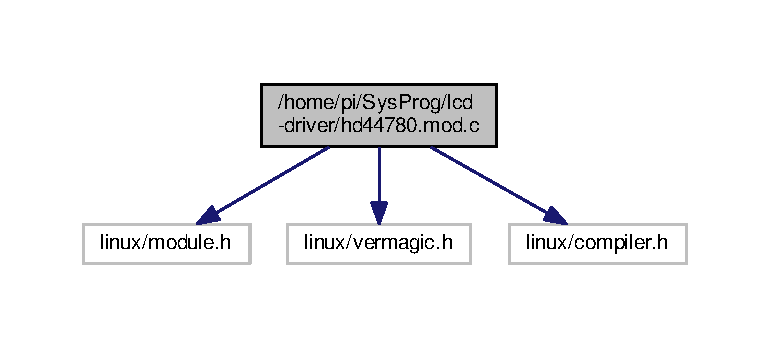
\includegraphics[width=350pt]{hd44780_8mod_8c__incl}
\end{center}
\end{figure}
\subsection*{Functions}
\begin{DoxyCompactItemize}
\item 
\hyperlink{hd44780_8mod_8c_a59ae061e50f755cbc9dbde3c6688273a}{M\+O\+D\+U\+L\+E\+\_\+\+I\+N\+F\+O} (vermagic, V\+E\+R\+M\+A\+G\+I\+C\+\_\+\+S\+T\+R\+I\+N\+G)
\item 
\+\_\+\+\_\+visible struct module \\*
\+\_\+\+\_\+this\+\_\+module \hyperlink{hd44780_8mod_8c_acc22bca8fb9ed0433181b5c98efdb5a4}{\+\_\+\+\_\+attribute\+\_\+\+\_\+} ((section(\char`\"{}.gnu.\+linkonce.\+this\+\_\+module\char`\"{})))
\item 
\hyperlink{hd44780_8mod_8c_a56679835ce5b854b84cd41c04545ac53}{M\+O\+D\+U\+L\+E\+\_\+\+I\+N\+F\+O} (srcversion,\char`\"{}4455\+E1\+A\+D6\+A5\+A9\+B806012607\char`\"{})
\end{DoxyCompactItemize}


\subsection{Function Documentation}
\hypertarget{hd44780_8mod_8c_acc22bca8fb9ed0433181b5c98efdb5a4}{\index{hd44780.\+mod.\+c@{hd44780.\+mod.\+c}!\+\_\+\+\_\+attribute\+\_\+\+\_\+@{\+\_\+\+\_\+attribute\+\_\+\+\_\+}}
\index{\+\_\+\+\_\+attribute\+\_\+\+\_\+@{\+\_\+\+\_\+attribute\+\_\+\+\_\+}!hd44780.\+mod.\+c@{hd44780.\+mod.\+c}}
\subsubsection[{\+\_\+\+\_\+attribute\+\_\+\+\_\+}]{\setlength{\rightskip}{0pt plus 5cm}\+\_\+\+\_\+visible struct module \+\_\+\+\_\+this\+\_\+module \+\_\+\+\_\+attribute\+\_\+\+\_\+ (
\begin{DoxyParamCaption}
\item[{(section(\char`\"{}.gnu.\+linkonce.\+this\+\_\+module\char`\"{}))}]{}
\end{DoxyParamCaption}
)}}\label{hd44780_8mod_8c_acc22bca8fb9ed0433181b5c98efdb5a4}
\hypertarget{hd44780_8mod_8c_a59ae061e50f755cbc9dbde3c6688273a}{\index{hd44780.\+mod.\+c@{hd44780.\+mod.\+c}!M\+O\+D\+U\+L\+E\+\_\+\+I\+N\+F\+O@{M\+O\+D\+U\+L\+E\+\_\+\+I\+N\+F\+O}}
\index{M\+O\+D\+U\+L\+E\+\_\+\+I\+N\+F\+O@{M\+O\+D\+U\+L\+E\+\_\+\+I\+N\+F\+O}!hd44780.\+mod.\+c@{hd44780.\+mod.\+c}}
\subsubsection[{M\+O\+D\+U\+L\+E\+\_\+\+I\+N\+F\+O}]{\setlength{\rightskip}{0pt plus 5cm}M\+O\+D\+U\+L\+E\+\_\+\+I\+N\+F\+O (
\begin{DoxyParamCaption}
\item[{vermagic}]{, }
\item[{V\+E\+R\+M\+A\+G\+I\+C\+\_\+\+S\+T\+R\+I\+N\+G}]{}
\end{DoxyParamCaption}
)}}\label{hd44780_8mod_8c_a59ae061e50f755cbc9dbde3c6688273a}
\hypertarget{hd44780_8mod_8c_a56679835ce5b854b84cd41c04545ac53}{\index{hd44780.\+mod.\+c@{hd44780.\+mod.\+c}!M\+O\+D\+U\+L\+E\+\_\+\+I\+N\+F\+O@{M\+O\+D\+U\+L\+E\+\_\+\+I\+N\+F\+O}}
\index{M\+O\+D\+U\+L\+E\+\_\+\+I\+N\+F\+O@{M\+O\+D\+U\+L\+E\+\_\+\+I\+N\+F\+O}!hd44780.\+mod.\+c@{hd44780.\+mod.\+c}}
\subsubsection[{M\+O\+D\+U\+L\+E\+\_\+\+I\+N\+F\+O}]{\setlength{\rightskip}{0pt plus 5cm}M\+O\+D\+U\+L\+E\+\_\+\+I\+N\+F\+O (
\begin{DoxyParamCaption}
\item[{srcversion}]{, }
\item[{\char`\"{}4455\+E1\+A\+D6\+A5\+A9\+B806012607\char`\"{}}]{}
\end{DoxyParamCaption}
)}}\label{hd44780_8mod_8c_a56679835ce5b854b84cd41c04545ac53}

\hypertarget{ioctl__header_8h}{\section{/home/pi/\+Sys\+Prog/lcd-\/driver/ioctl\+\_\+header.h File Reference}
\label{ioctl__header_8h}\index{/home/pi/\+Sys\+Prog/lcd-\/driver/ioctl\+\_\+header.\+h@{/home/pi/\+Sys\+Prog/lcd-\/driver/ioctl\+\_\+header.\+h}}
}
{\ttfamily \#include $<$linux/ioctl.\+h$>$}\\*
Include dependency graph for ioctl\+\_\+header.\+h\+:\nopagebreak
\begin{figure}[H]
\begin{center}
\leavevmode
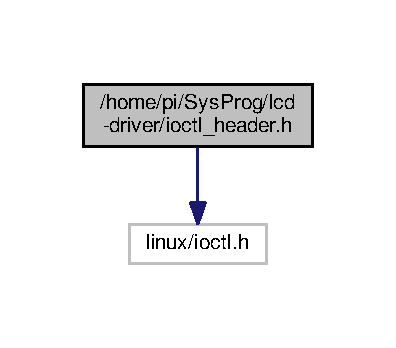
\includegraphics[width=190pt]{ioctl__header_8h__incl}
\end{center}
\end{figure}
This graph shows which files directly or indirectly include this file\+:\nopagebreak
\begin{figure}[H]
\begin{center}
\leavevmode
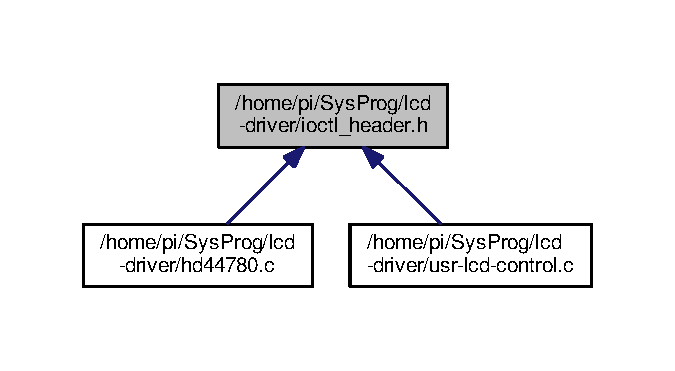
\includegraphics[width=350pt]{ioctl__header_8h__dep__incl}
\end{center}
\end{figure}
\subsection*{Macros}
\begin{DoxyCompactItemize}
\item 
\#define \hyperlink{ioctl__header_8h_a23f15b5855019d8ac0c75f82484f8047}{M\+A\+G\+I\+C\+\_\+\+N\+U\+M}~'k' 	/$\ast$unique arbitrary number for driver$\ast$/
\item 
\#define \hyperlink{ioctl__header_8h_a85699dc8e51a8445392801b9e1994758}{I\+O\+C\+T\+L}~\+\_\+\+I\+O(\hyperlink{ioctl__header_8h_a23f15b5855019d8ac0c75f82484f8047}{M\+A\+G\+I\+C\+\_\+\+N\+U\+M}, 0);		/$\ast$int argument$\ast$/
\item 
\#define \hyperlink{ioctl__header_8h_a7397849fd9ac3e2bc321921033aae806}{I\+O\+C\+T\+L\+\_\+\+W\+R\+I\+T\+E}~\+\_\+\+I\+O\+W(\hyperlink{ioctl__header_8h_a23f15b5855019d8ac0c75f82484f8047}{M\+A\+G\+I\+C\+\_\+\+N\+U\+M}, 2, int)		/$\ast$returns sizeof(int) bytes to the user $\ast$/
\item 
\#define \hyperlink{ioctl__header_8h_a8cbb4cc1fd96df34b3e16eb1ea744455}{I\+O\+C\+T\+L\+\_\+\+R\+E\+A\+D}~\+\_\+\+I\+O\+R(\hyperlink{ioctl__header_8h_a23f15b5855019d8ac0c75f82484f8047}{M\+A\+G\+I\+C\+\_\+\+N\+U\+M}, 3, int)		/$\ast$...$\ast$/
\end{DoxyCompactItemize}


\subsection{Macro Definition Documentation}
\hypertarget{ioctl__header_8h_a85699dc8e51a8445392801b9e1994758}{\index{ioctl\+\_\+header.\+h@{ioctl\+\_\+header.\+h}!I\+O\+C\+T\+L@{I\+O\+C\+T\+L}}
\index{I\+O\+C\+T\+L@{I\+O\+C\+T\+L}!ioctl\+\_\+header.\+h@{ioctl\+\_\+header.\+h}}
\subsubsection[{I\+O\+C\+T\+L}]{\setlength{\rightskip}{0pt plus 5cm}\#define I\+O\+C\+T\+L~\+\_\+\+I\+O({\bf M\+A\+G\+I\+C\+\_\+\+N\+U\+M}, 0);		/$\ast$int argument$\ast$/}}\label{ioctl__header_8h_a85699dc8e51a8445392801b9e1994758}
\hypertarget{ioctl__header_8h_a8cbb4cc1fd96df34b3e16eb1ea744455}{\index{ioctl\+\_\+header.\+h@{ioctl\+\_\+header.\+h}!I\+O\+C\+T\+L\+\_\+\+R\+E\+A\+D@{I\+O\+C\+T\+L\+\_\+\+R\+E\+A\+D}}
\index{I\+O\+C\+T\+L\+\_\+\+R\+E\+A\+D@{I\+O\+C\+T\+L\+\_\+\+R\+E\+A\+D}!ioctl\+\_\+header.\+h@{ioctl\+\_\+header.\+h}}
\subsubsection[{I\+O\+C\+T\+L\+\_\+\+R\+E\+A\+D}]{\setlength{\rightskip}{0pt plus 5cm}\#define I\+O\+C\+T\+L\+\_\+\+R\+E\+A\+D~\+\_\+\+I\+O\+R({\bf M\+A\+G\+I\+C\+\_\+\+N\+U\+M}, 3, int)		/$\ast$...$\ast$/}}\label{ioctl__header_8h_a8cbb4cc1fd96df34b3e16eb1ea744455}
\hypertarget{ioctl__header_8h_a7397849fd9ac3e2bc321921033aae806}{\index{ioctl\+\_\+header.\+h@{ioctl\+\_\+header.\+h}!I\+O\+C\+T\+L\+\_\+\+W\+R\+I\+T\+E@{I\+O\+C\+T\+L\+\_\+\+W\+R\+I\+T\+E}}
\index{I\+O\+C\+T\+L\+\_\+\+W\+R\+I\+T\+E@{I\+O\+C\+T\+L\+\_\+\+W\+R\+I\+T\+E}!ioctl\+\_\+header.\+h@{ioctl\+\_\+header.\+h}}
\subsubsection[{I\+O\+C\+T\+L\+\_\+\+W\+R\+I\+T\+E}]{\setlength{\rightskip}{0pt plus 5cm}\#define I\+O\+C\+T\+L\+\_\+\+W\+R\+I\+T\+E~\+\_\+\+I\+O\+W({\bf M\+A\+G\+I\+C\+\_\+\+N\+U\+M}, 2, int)		/$\ast$returns sizeof(int) bytes to the user $\ast$/}}\label{ioctl__header_8h_a7397849fd9ac3e2bc321921033aae806}
\hypertarget{ioctl__header_8h_a23f15b5855019d8ac0c75f82484f8047}{\index{ioctl\+\_\+header.\+h@{ioctl\+\_\+header.\+h}!M\+A\+G\+I\+C\+\_\+\+N\+U\+M@{M\+A\+G\+I\+C\+\_\+\+N\+U\+M}}
\index{M\+A\+G\+I\+C\+\_\+\+N\+U\+M@{M\+A\+G\+I\+C\+\_\+\+N\+U\+M}!ioctl\+\_\+header.\+h@{ioctl\+\_\+header.\+h}}
\subsubsection[{M\+A\+G\+I\+C\+\_\+\+N\+U\+M}]{\setlength{\rightskip}{0pt plus 5cm}\#define M\+A\+G\+I\+C\+\_\+\+N\+U\+M~'k' 	/$\ast$unique arbitrary number for driver$\ast$/}}\label{ioctl__header_8h_a23f15b5855019d8ac0c75f82484f8047}
I\+O\+C\+T\+L creates a kernelmessage I\+O\+C\+T\+L\+\_\+\+W\+R\+I\+T\+E writes a variable to the character driver and also prints a kernel message I\+O\+C\+T\+L\+\_\+\+R\+E\+A\+D reads a variable from the driver 
\hypertarget{README_8md}{\section{/home/pi/\+Sys\+Prog/lcd-\/driver/\+R\+E\+A\+D\+M\+E.md File Reference}
\label{README_8md}\index{/home/pi/\+Sys\+Prog/lcd-\/driver/\+R\+E\+A\+D\+M\+E.\+md@{/home/pi/\+Sys\+Prog/lcd-\/driver/\+R\+E\+A\+D\+M\+E.\+md}}
}

\hypertarget{usr-lcd-control_8c}{\section{/home/pi/\+Sys\+Prog/lcd-\/driver/usr-\/lcd-\/control.c File Reference}
\label{usr-lcd-control_8c}\index{/home/pi/\+Sys\+Prog/lcd-\/driver/usr-\/lcd-\/control.\+c@{/home/pi/\+Sys\+Prog/lcd-\/driver/usr-\/lcd-\/control.\+c}}
}


a linux user space program that communicates with the hd44780 linux kernel module (L\+K\+M). to work with the device the /dev/hd44780 must be called  


{\ttfamily \#include $<$stdio.\+h$>$}\\*
{\ttfamily \#include $<$fcntl.\+h$>$}\\*
{\ttfamily \#include $<$errno.\+h$>$}\\*
{\ttfamily \#include $<$unistd.\+h$>$}\\*
{\ttfamily \#include $<$stdlib.\+h$>$}\\*
{\ttfamily \#include $<$string.\+h$>$}\\*
{\ttfamily \#include $<$ctype.\+h$>$}\\*
{\ttfamily \#include \char`\"{}ioctl\+\_\+header.\+h\char`\"{}}\\*
Include dependency graph for usr-\/lcd-\/control.c\+:\nopagebreak
\begin{figure}[H]
\begin{center}
\leavevmode
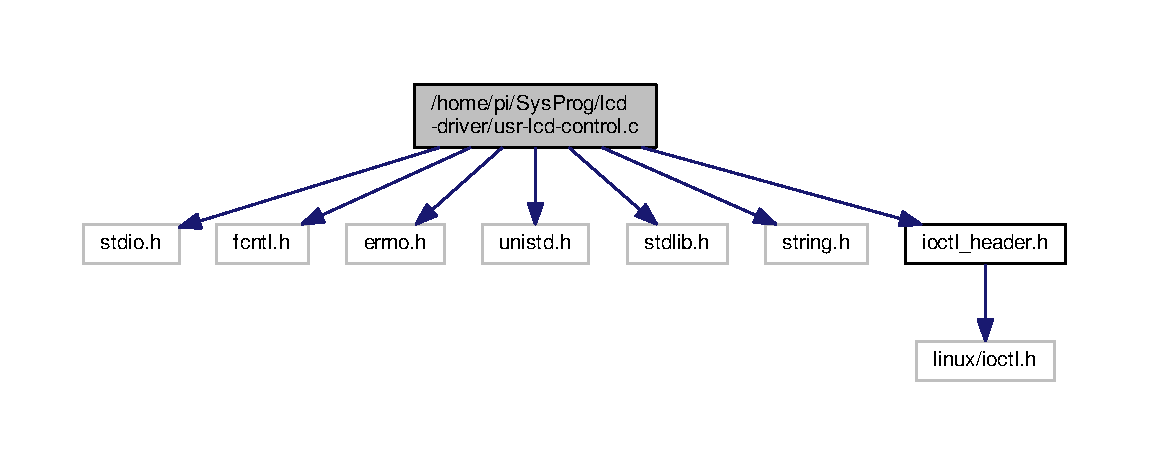
\includegraphics[width=350pt]{usr-lcd-control_8c__incl}
\end{center}
\end{figure}
\subsection*{Functions}
\begin{DoxyCompactItemize}
\item 
int \hyperlink{usr-lcd-control_8c_a3c04138a5bfe5d72780bb7e82a18e627}{main} (int argc, char $\ast$$\ast$argv)
\end{DoxyCompactItemize}


\subsection{Detailed Description}
a linux user space program that communicates with the hd44780 linux kernel module (L\+K\+M). to work with the device the /dev/hd44780 must be called 

\begin{DoxyAuthor}{Author}
Daniel Obermaier 
\end{DoxyAuthor}
\begin{DoxyDate}{Date}
02.\+06.\+2016 
\end{DoxyDate}
\begin{DoxyVersion}{Version}
0.\+1 
\end{DoxyVersion}


\subsection{Function Documentation}
\hypertarget{usr-lcd-control_8c_a3c04138a5bfe5d72780bb7e82a18e627}{\index{usr-\/lcd-\/control.\+c@{usr-\/lcd-\/control.\+c}!main@{main}}
\index{main@{main}!usr-\/lcd-\/control.\+c@{usr-\/lcd-\/control.\+c}}
\subsubsection[{main}]{\setlength{\rightskip}{0pt plus 5cm}int main (
\begin{DoxyParamCaption}
\item[{int}]{argc, }
\item[{char $\ast$$\ast$}]{argv}
\end{DoxyParamCaption}
)}}\label{usr-lcd-control_8c_a3c04138a5bfe5d72780bb7e82a18e627}

\begin{DoxyCode}
22                                \{
23 
24 \textcolor{keyword}{static} \textcolor{keyword}{const} \textcolor{keywordtype}{char}* devname = \textcolor{stringliteral}{"/dev/hd44780"};
25 
26 \textcolor{keywordtype}{int} ret = 0;
27 \textcolor{keywordtype}{char} buff[128] = \textcolor{stringliteral}{""};
28 \textcolor{keywordtype}{int} \hyperlink{hd44780_8c_a8910285a0352a5c710e65ec9ecbe32a1}{dev} = 0;
29 
30 \textcolor{keywordflow}{if}(argc != 2)\{ \textcolor{comment}{/*argc should be 2 for correct execution*/}
31     printf(\textcolor{stringliteral}{"usage:  <filename> <string>\(\backslash\)n"});
32 \}
33 \textcolor{keywordflow}{else}\{
34     \textcolor{comment}{//assume argv[1] is the string to write }
35     \textcolor{keywordtype}{int} dev = open(devname, O\_WRONLY);  \textcolor{comment}{//open device file -> WRITE ONLY}
36     
37     ret = write(dev, \textcolor{stringliteral}{"                                "}, 32);   \textcolor{comment}{//clear display}
38     \textcolor{keywordflow}{if}(dev == -1)\{
39         perror(\textcolor{stringliteral}{"can't open device file\(\backslash\)n"});
40         \textcolor{keywordflow}{return} -EIO;
41     \}
42 
43     ret = write(dev, argv[1], 128); \textcolor{comment}{//write string to device}
44 
45     \textcolor{keywordflow}{if}(ret < 0)\{
46         perror(\textcolor{stringliteral}{"cant write to devicefile\(\backslash\)n"});
47         \textcolor{keywordflow}{return} EIO;
48     \}
49 \}
50 
51 close(dev);     \textcolor{comment}{//close device afterwards}
52 
53 \textcolor{keywordflow}{return} 0;
54 \}
\end{DoxyCode}

%--- End generated contents ---

% Index
\newpage
\phantomsection
\addcontentsline{toc}{chapter}{Index}
\printindex

\end{document}
